\documentclass{scrbook}


% FSFW-LaTeX-Vorlage
% VERSION = 0.2 (2016-10-16)


% Alle Zeilen die mit % anfangen sind Kommentare
% In TeXstudio kann man eine oder mehrere Zeilen mit STRG+T in einen Kommentar
% verwandeln. STRG+U ist die Umkehrung (zu finden im Menü "Idefix").
% Das ist sehr praktisch beim Suchen von Fehlern: Alles wo der Fehler stecken
% könnte auskommentieren bis es funktioniert und dann schrittweise wieder
% "einkommentieren" bis der Fehler auftritt. 

% Wichtiger Hinweis: diese Vorlage nutzt zur Erstellung des
% Literaturverzeichnisses das Program "biber" anstatt des älteren "bibtex" .
% Falls es Probleme beim kompilieren gibt, bitte prüfen, ob biber korrekt
% ausgeführt wurde.



\usepackage[ngerman]{babel}
\usepackage[T1]{fontenc}
\usepackage[utf8]{inputenc}

% Paket für interne verlinkungen
\usepackage{hyperref}

% mögliche Angaben für Farben, siehe z.B.
% http://tex.stackexchange.com/questions/50747/options-for-appearance-of-links-in-hyperref
\hypersetup{
colorlinks=true,
allcolors=[rgb]{0, .1, .5} % dunkelblau
%allcolors=[rgb]{0, 0, 0} % schwarz
}

\usepackage{csquotes}
\MakeAutoQuote{„}{“}
\usepackage{cleveref}

\usepackage[scale=0.95]{tgpagella}
\usepackage[scale=0.92]{tgheros}

% diese Schriftart sieht zwar schön aus ist aber im Paket
% texlive-fonts-extra welches sehr groß ist.
\usepackage[scaled=0.83]{beramono}

\usepackage{mathpazo}

\setlength{\parindent}{0cm}
\setlength{\parskip}{0.5ex}

\usepackage[style=authoryear,backend=biber]{biblatex}

% hier wird die Datei eingebunden, in der alle möglichen Quellen stehen können.
\addbibresource{literatur.bib}

% LaTeX und biber sorgen dann dafür, dass nur die zitierten Quellen auch im
% Literaturverzeichnis auftauchen

\usepackage{makeidx}
\makeindex

\usepackage{tabu}
\usepackage{booktabs}

\usepackage{mathtools}
\newtheorem{Satz}{Satz}

\usepackage{todonotes}

\begin{document}

\frontmatter

\begin{titlepage}

  \begin{center}
    \Huge

    Technische Universität Dresden

    Fachrichtung Zukunfswissenschaften

    \bigskip

    \LARGE

    Institut für Höhere Kognition

    \vfill

    \huge

    \textbf{Über das Sein und Nichtsein von\\ Werden und Vergehen}

    \LARGE

    \vfill

    Diplomarbeit \\
    zur Erlangung des ersten akademischen Grades

    \bigskip

    \textbf{Diplomakademikerin}

  \end{center}

  \vfill

  \Large

  vorgelegt von

  \vspace*{2\bigskipamount}

  \begin{tabular}{@{}lp{4cm}@{\qquad}rl@{}}
    Name:       & Lustig     & Vorname: & Lutetia\\[2.0ex]
    geboren am: & 17.03.1976 & in:      & Duckburg
  \end{tabular}

  \vspace*{4\bigskipamount}

  Tag der Einreichung: 29.02.2016

  \vspace*{2\bigskipamount}

  Betreuer: Prof. Dr. nihil. Siegfried von Gestern

\end{titlepage}

\newpage

\hbox{}\vfill

\noindent
Copyright \copyright\  2016 Lutetia Lustig\\
This work is licensed under the Creative Commons Attribution-ShareAlike 4.0
International License. To view a copy of this license, visit
\url{http://creativecommons.org/licenses/by-sa/4.0/deed.en_US}.

\chapter*{Vorwort}

In unserer virtuellen Zeit ist es wichtiger denn je, sich des Unterschieds
zwischen dem Hier und dem Jetzt klar zu werden.  Eine einfacher Verwischung
dieser beiden doch sehr unterschiedlichen Begriffe kann dafür sorgen, dass wir
uns in unserem Denken und Handeln nicht mehr leiten lassen von den Motivation
unser Intuition, sondern von der Versprechungen der externen Welt.  Ein Teil
dieser Arbeit soll es sein, sich diesen Begrifflichkeiten auf wissenschaftlichem
Wege zu nähern und so auch für die Außenstehende und den Außenstehenden klar zu
machen, was die Kerngedanken in der Unterscheidung von Hier und Jetzt sind.

Die Arbeit lässt sich grob in drei Teile gliedern.  In \Cref{cha:eins} befassen
wir uns mit den Grundbegrifflichkeiten der modernen Wesenslehre.  In
\ref{cha:zwei} ziehen wir erst Verbindungen zu Beobachtungen aus der realen
Welt, und in \Cref{cha:drei} schließlich führen wir die Ergebnisse der
vorherigen Abschnitte in einer kontroversen Argumentationsstruktur zusammen.

\cleardoublepage

\tableofcontents

\mainmatter

\chapter{Eins, \dots}
\label{cha:eins}

Es geht los, seien Sie gespannt!

\section{Der erste Streich!}
\label{sec:der-erste-streich}

Wir beginnen mit einer einfach Betrachtung klassischer Beispiele.  Dafür
verweisen wir zuerst eloquent auf die folgende Tabelle verweisen:\index{Tabelle}

\begin{center}
  \begin{tabu}{XX}
    \toprule
    Begriff & Bedeutung \\\midrule
    Sein des Wesens und des Geistes & Die Quintessenz aller Dinge \\
    Nichtsein als Verständnis des Nichts & Das Antonym des Wesean \\
    \bottomrule
  \end{tabu}
\end{center}

\section{Und der zweite folgt sogleich!}
\label{sec:und-der-zweite}

Diese Begrifflichkeiten entziehen sich nicht einer bestimmten Mystik, die sie
seit ihrer Entstehung in der Wiege der menschlichen Gedankenwelt genießen.  Eine
ebenso wichtige Begrifflichkeit mit nicht weniger Mystik sind die
\emph{Primzahlen}, die für diese Arbeit zwar nicht relevant sind, aber dennoch
in keiner Arbeit fehlen dürfen!  Wir zeigen die ersten 10000 Primzahlen in
\Cref{tab:prime-numbers}.

\begin{table}[tp]
  \centering
  \begin{tabu}{XXXXXXXXXX}
    \toprule
      2 &    3 &    5 &    7 &   11 &   13 &   17 &   19 &   23 &   29 \\
     31 &   37 &   41 &   43 &   47 &   53 &   59 &   61 &   67 &   71 \\
     73 &   79 &   83 &   89 &   97 &  101 &  103 &  107 &  109 &  113 \\
    127 &  131 &  137 &  139 &  149 &  151 &  157 &  163 &  167 &  173 \\
    179 &  181 &  191 &  193 &  197 &  199 &  211 &  223 &  227 &  229 \\
    233 &  239 &  241 &  251 &  257 &  263 &  269 &  271 &  277 &  281 \\
    283 &  293 &  307 &  311 &  313 &  317 &  331 &  337 &  347 &  349 \\
    353 &  359 &  367 &  373 &  379 &  383 &  389 &  397 &  401 &  409 \\
    419 &  421 &  431 &  433 &  439 &  443 &  449 &  457 &  461 &  463 \\
    467 &  479 &  487 &  491 &  499 &  503 &  509 &  521 &  523 &  541 \\
    547 &  557 &  563 &  569 &  571 &  577 &  587 &  593 &  599 &  601 \\
    607 &  613 &  617 &  619 &  631 &  641 &  643 &  647 &  653 &  659 \\
    661 &  673 &  677 &  683 &  691 &  701 &  709 &  719 &  727 &  733 \\
    739 &  743 &  751 &  757 &  761 &  769 &  773 &  787 &  797 &  809 \\
    811 &  821 &  823 &  827 &  829 &  839 &  853 &  857 &  859 &  863 \\
    877 &  881 &  883 &  887 &  907 &  911 &  919 &  929 &  937 &  941 \\
    947 &  953 &  967 &  971 &  977 &  983 &  991 &  997 & 1009 & 1013 \\
   1019 & 1021 & 1031 & 1033 & 1039 & 1049 & 1051 & 1061 & 1063 & 1069 \\
   1087 & 1091 & 1093 & 1097 & 1103 & 1109 & 1117 & 1123 & 1129 & 1151 \\
   1153 & 1163 & 1171 & 1181 & 1187 & 1193 & 1201 & 1213 & 1217 & 1223 \\
   1229 & 1231 & 1237 & 1249 & 1259 & 1277 & 1279 & 1283 & 1289 & 1291 \\
   1297 & 1301 & 1303 & 1307 & 1319 & 1321 & 1327 & 1361 & 1367 & 1373 \\
   1381 & 1399 & 1409 & 1423 & 1427 & 1429 & 1433 & 1439 & 1447 & 1451 \\
   1453 & 1459 & 1471 & 1481 & 1483 & 1487 & 1489 & 1493 & 1499 & 1511 \\
   1523 & 1531 & 1543 & 1549 & 1553 & 1559 & 1567 & 1571 & 1579 & 1583 \\
   1597 & 1601 & 1607 & 1609 & 1613 & 1619 & 1621 & 1627 & 1637 & 1657 \\
   1663 & 1667 & 1669 & 1693 & 1697 & 1699 & 1709 & 1721 & 1723 & 1733 \\
   1741 & 1747 & 1753 & 1759 & 1777 & 1783 & 1787 & 1789 & 1801 & 1811 \\
   1823 & 1831 & 1847 & 1861 & 1867 & 1871 & 1873 & 1877 & 1879 & 1889 \\
   1901 & 1907 & 1913 & 1931 & 1933 & 1949 & 1951 & 1973 & 1979 & 1987 \\
   1993 & 1997 & 1999 & 2003 & 2011 & 2017 & 2027 & 2029 & 2039 & 2053 \\
   2063 & 2069 & 2081 & 2083 & 2087 & 2089 & 2099 & 2111 & 2113 & 2129 \\
   2131 & 2137 & 2141 & 2143 & 2153 & 2161 & 2179 & 2203 & 2207 & 2213 \\
   2221 & 2237 & 2239 & 2243 & 2251 & 2267 & 2269 & 2273 & 2281 & 2287 \\
   2293 & 2297 & 2309 & 2311 & 2333 & 2339 & 2341 & 2347 & 2351 & 2357 \\
   2371 & 2377 & 2381 & 2383 & 2389 & 2393 & 2399 & 2411 & 2417 & 2423 \\
   \bottomrule
  \end{tabu}
  \caption{Die ersten 10000 Primzahlen (nicht ganz \dots)\index{Primzahlen}}
  \label{tab:prime-numbers}
\end{table}

\section{Das War's}
\label{sec:das-wars}

Damit ist schon das wichtigste dieses Abschnittes gesagt.  Alles weitere findet
sich in~\cite{lakoff87_women_fire_danger_thing}.

\chapter{\dots, Zwei, \dots}
\label{cha:zwei}

Eine allgemein anerkannte Weisheit besagt, dass alles stimmt, was sich in
mathematischen Formeln ausdrücken lässt.  Um also den in dieser Arbeit gegebenen
Thesen noch mehr Gewicht zu geben, weisen wir hier unterstützend nach, dass sie
aus bekannt Formel der Höheren Mathematik folgen.

\section{Vorbereitungen}
\label{sec:vorbereitungen}

Zuerst wollen wir aber einige wichtige Formeln der Mathematik nennen.

Als einer der ästhetisch ansprechendsten Formel gilt
\begin{equation}
  \label{eq:1}
  e^{i\pi} + 1 = 0.
\end{equation}
Diese Formel hat nur leider nichts mit dem zu tun, worum es in dieser Arbeit
gehen soll.  Ebenso ist es mit dem folgenden \emph{Cauchyschen
  Integralsatz}~\parencite{knopp70_funkt_i}.\index{Mathematik}\index{Hauptsatz}

\begin{Satz}[Hauptsatz der Funktionentheorie]
  Es sei die Funktion $f$ in einem einfach zusammenhängenden Gebiet
  $\mathcal{G}$, und es seien $z_{0}$ und $Z$ zwei innere Punkte von
  $\mathcal{G}$.  Dann hat das Integral
  \begin{equation*}
    \int_{z_{0}}^{Z} \! f(z) \; \mathrm{d}z
  \end{equation*}
  längs jeden von $z_{0}$ nach $Z$ führenden in ganz in $\mathcal{G}$
  verlaufenden Weges denselben Wert.
\end{Satz}

\section{Ergebnisse}
\label{sec:ergebnisse}

Es zeigt, dass auch nach vertiefter Untersuchung sich keinerlei Verbindungen
zwischen der Mathematik auf der einen, und der in dieser Arbeit beschriebenen
Thematik auf der anderen Seite finden lassen.  Dennoch sein darauf hingewiesen,
dass dies in keiner Weise die Glaubwürdigkeit der angebrachten Argumente in
irgendeiner Weise angreift!

\chapter{\dots, Drei!}
\label{cha:drei}

Keine Arbeit kann vollständig sein ohne eine eingebundene Graphik, und sei sie
noch so unabhängig vom eigentlichen Anliegen des Werkes.  Nun denn, hier ist
sie:\index{Abbildung}

\begin{figure}[h]
  \centering
  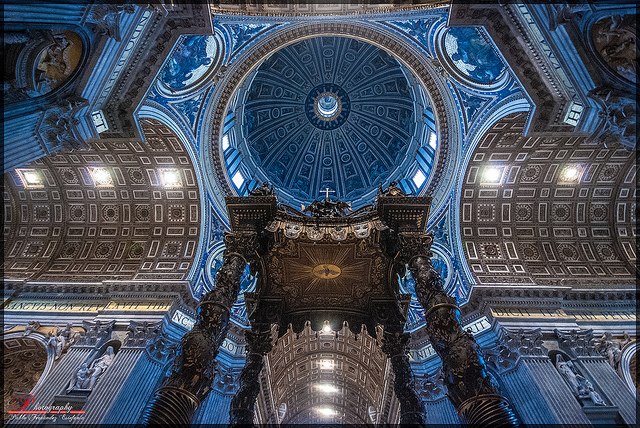
\includegraphics[width=\linewidth]{eyes-to-heaven.jpg}
  \caption{„Eyes to Heaven“, Basílica de San Pedro, Vatikan, Italien,
    CC-BY-NC-ND Pablo Fernández,
    \url{https://www.flickr.com/photos/hadock/8449312293/} }
  \label{fig:basilica-de-san-pedro}
\end{figure}

\appendix

\chapter{Dinge, die noch gesagt werden müssen}
\label{cha:dinge-die-noch}

Tatsächlich fällt mir doch noch was ein, und zwar ein Zitat\index{Zitat}:

\begin{displayquote}[Richard Feynman]
  „The first principle is that you must not fool yourself – and you are the
  easiest person to fool.“
\end{displayquote}

\section{Weitere Informationen}
Fragen und Probleme rund um LaTeX können in der FSFW-Sprechstunde geklärt werden: 
\url{https://fsfw-dresden.de/sprechstunde}.

\backmatter

\printbibliography{}

\printindex

\cleardoublepage

\thispagestyle{empty}

\hbox{}\vfill

\textbf{\large ERKLÄRUNG}

\bigskip \medskip

Hiermit erkläre ich, dass ich die am heutigen Tag eingereichte Diplomarbeit zum
Thema „Über das Sein und Nichtsein von Werden und Vergehen“ unter Betreuung von
Prof.~Dr.~nihil.~Siegfried von Gestern selbstständig erarbeitet, verfasst und
Zitate kenntlich gemacht habe. Andere als die angegebenen Hilfsmittel wurden von
mir nicht benutzt.

\vspace*{5\bigskipamount}

Datum \hfill Unterschrift

\normalsize

\vspace*{2\bigskipamount}

\vfill\hbox{}

\end{document}
